\documentclass{article}
\usepackage{amsmath, amssymb, amsfonts, amsthm}
\usepackage{cancel}
\usepackage[output-complex-root=j]{siunitx}
\usepackage[american, nooldvoltagedirection]{circuitikz}
\usepackage{bm}
\usepackage{listings}
\usepackage{graphicx}
\usepackage{fullpage}
\usepackage{hyperref}

\renewcommand{\thesection}{\arabic{section}}
\renewcommand{\thesubsection}{\thesection.\alph{subsection}}
\renewcommand{\thesubsubsection}{\thesubsection.\roman{subsubsection}}

\newtheorem{theorem}{Theorem}
\DeclareSIUnit\year{yr}
\DeclareSIUnit\parsec{pc}

\newcommand{\unit}[1]{\bm{\hat{#1}}}
\newcommand{\iprod}[2]{\left\langle #1, #2 \right\rangle}
\newcommand{\tpose}[1]{\left[#1\right]^{\! \top} \!\!}
\newcommand{\diff}[1]{\frac{d}{d #1}}

\lstset{
    language=Python,
    tabsize=4,
    basicstyle=\ttfamily,
    numbers=left,
    numberstyle=\ttfamily,
    keywordstyle=\color{blue},
    frame=single
}

\title{ASTRO7A PS02}
\author{Bryan Ngo}
\date{2020-09-07}

\begin{document}

\maketitle

\section{Sunlight in Berkeley}

\subsection{}

\begin{center}
    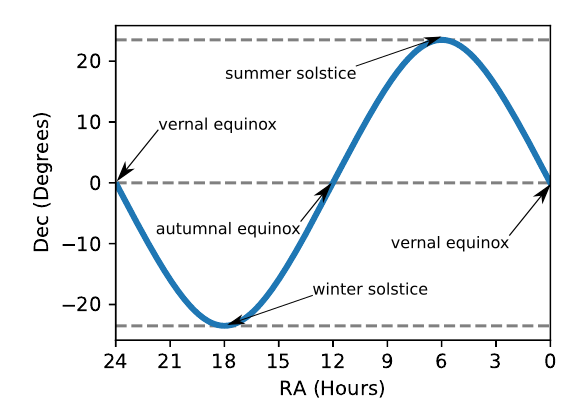
\includegraphics[width=0.8\textwidth]{q1a.png}
\end{center}

\subsection{}

The formula for altitude is
\begin{equation}
    d = \SI{90}{\degree} - d_{\text{Berk}} \pm \SI{23.5}{\degree}
\end{equation}
where the sign of Earth's tilt depends on whether it is at the winter or summer solstice.
\begin{center}
    \begin{tabular}{||c|c||}
        \hline
        Position & Altitude \\
        \hline
        Vernal Equinox & \SI{52.13}{\degree} \\
        Winter Solstice & \SI{28.63}{\degree} \\
        Autumnal Equinox & \SI{52.13}{\degree} \\
        Summer Solstice & \SI{75.63}{\degree} \\
        \hline
    \end{tabular}
\end{center}

\subsection{}

If there was a \SI{42}{\degree} orbital tilt, the sun's ecliptic would make a sharper angle with the orbital plane than it currently does.
This means that at the solstices, the Sun will appear higher in the sky.
The equinoxes will not change since the Sun intersects the orbital plane at these points.
In the context of the ecliptic sine wave, the amplitude will increase, meaning the absolute value of the maximum is now \SI{42}{\degree}.
The new altitudes are
\begin{center}
    \begin{tabular}{||c|c||}
        \hline
        Position & Altitude \\
        \hline
        Vernal Equinox & \SI{52.13}{\degree} \\
        Winter Solstice & \SI{10.13}{\degree} \\
        Autumnal Equinox & \SI{52.13}{\degree} \\
        Summer Solstice & \SI{94.13}{\degree} \\
        \hline
    \end{tabular}
\end{center}

\section{A Compact Planetary System}

\subsection{}

The generalized formula of Kepler's third law with units of astronomical units and days is
\begin{equation}
    \left(\frac{P}{365}\right)^2 = a^3 \implies a = \left(\frac{P}{365}\right)^{\frac{2}{3}}
\end{equation}
From there, we can use the equation to determine the periastron and apastron to be, respectively,
\begin{align}
    r_p &= \left.\frac{a (1 - e^2)}{1 + e \cos(\theta)}\right|_{\theta=0} = \frac{a (1 - e^2)}{1 + e} = a (1 - e) \label{eq:periastron} \\
    r_a &= \left.\frac{a (1 - e^2)}{1 + e \cos(\theta)}\right|_{\theta=\SI{\pi}{\radian}} = \frac{a (1 - e^2)}{1 - e} = a (1 + e) \label{eq:apastron}
\end{align}
\begin{center}
    \begin{tabular}{||c|c|c|c||}
        \hline
        Planet & Semimajor Axis [\si{\astronomicalunit}] & Periastron Distance [\si{\astronomicalunit}] & Apastron Distance [\si{\astronomicalunit}] \\
        \hline
        b & \num{9.27e-2} & \num{8.85e-2} & \num{9.69e-2} \\
        c & \num{1.10e-1} & \num{1.06e-1} & \num{1.11e-1} \\
        d & \num{1.57e-1} & \num{1.56e-1} & \num{1.58e-1} \\
        e & \num{1.97e-1} & \num{1.95e-1} & \num{2.00e-1} \\
        f & \num{2.54e-1} & \num{2.51e-1} & \num{2.57e-1} \\
        g & \num{4.72e-1} & \num{4.01e-1} & \num{5.43e-1} \\
        \hline
    \end{tabular}
\end{center}

\subsection{}

The two closest planets are planets b and c, with a closest approach distance of only \SI{9.1e-3}{\astronomicalunit}.

\subsection{}

Converting to SI units, our givens are
\begin{align}
    M_b &= 1.9 \cdot \SI{5.9722e+24}{\kilogram} = \SI{1.13e+25}{\kilogram} \\
    M_c &= 2.9 \cdot \SI{5.9722e+24}{\kilogram} = \SI{1.73e+25}{\kilogram} \\
    r_{bc} &= \frac{\SI{9.1e-3}{\cancel\astronomicalunit}}{1} \cdot \frac{\SI{149597870700}{\meter}}{\SI{1}{\cancel\astronomicalunit}} = \SI{1.36e+9}{\meter}
\end{align}
Then, using Newton's law of universal gravitation,
\begin{equation}
    F_{bc} = \frac{G M_b M_c}{r_{bc}^2} = \frac{G (\SI{1.13e+25}{\kilogram}) (\SI{1.73e+25}{\kilogram})}{(\SI{1.36e+9}{\meter})^2} = \SI{7.08e+21}{\newton}
\end{equation}

\subsection{}

Our givens are
\begin{align}
    M_\star &= 0.961 \cdot \SI{1.98847e+30}{\kilogram} = \SI{1.91e+30}{\kilogram}\\
    r_{b\star} &= \frac{\SI{9.69e-2}{\cancel\astronomicalunit}}{1} \cdot \frac{\SI{149597870700}{\meter}}{\SI{1}{\cancel\astronomicalunit}} = \SI{1.45e+10}{\meter}
\end{align}
The force between planet b and its sun is
\begin{equation}
    F_{b\star} = \frac{G M_B M_\star}{r_{b\star}^2} = \frac{G (\SI{1.13e+25}{\kilogram}) (\SI{1.91e+30}{\kilogram})}{(\SI{1.45e+10}{\meter})^2} = \SI{6.89e+24}{\newton}
\end{equation}
Meaning that the ratio between the closest approach and the solar attraction is
\begin{equation}
    \frac{F_{bc}}{F_{b\star}} = \num{1.03e-3}
\end{equation}

\subsection{}

Here, we want \(r_a\) of planet b to equal \(r_p\) of planet c.
Equating \autoref{eq:periastron} and \autoref{eq:apastron},
\begin{align}
    a_b (1 + e_b) &= a_c (1 - e_c) \\
    \Rightarrow e_b &= \frac{a_c}{a_b} (1 - e_c) - 1 \\
    &= 0.139
\end{align}
So the eccentricity increases by \SI{208}{\percent}.

\subsection{}

\begin{center}
    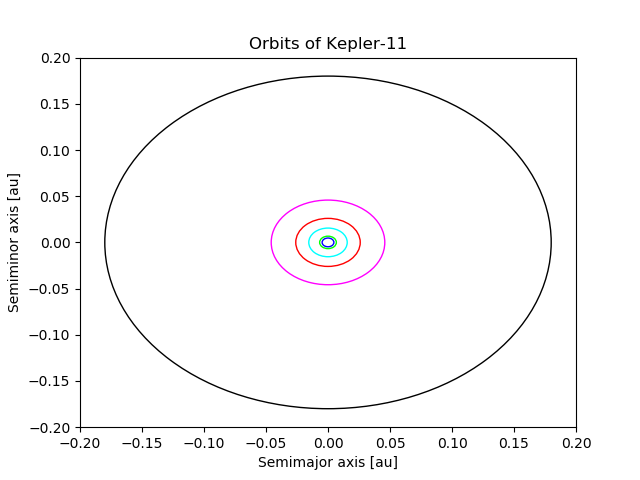
\includegraphics[width=0.8\textwidth]{q2f.png}
\end{center}

\section{Eccentric Comets}

\subsection{}

Using Kepler's third law,
\begin{equation}
    P^2 = a^3 \implies a = (\SI{6.45}{\year})^{\frac{2}{3}} = \SI{3.47}{\astronomicalunit}
\end{equation}

\subsection{}

Using \autoref{eq:periastron} and \autoref{eq:apastron},
\begin{align}
    r_p &= a (1 - e) = \SI{1.25}{\astronomicalunit} \\
    r_p &= a (1 + e) = \SI{5.68}{\astronomicalunit} \\
\end{align}

\subsection{}

\begin{equation}
    E_{tot} = \frac{1}{2} \mu v^2 - \frac{G M \mu}{r}
\end{equation}
where \(\mu = \frac{M_\odot m_{comet}}{M_\odot + m_{comet}}\) and \(M = M_\odot + m_{comet}\).
Equating the two expressions,
\begin{align}
    E_{tot} = \frac{1}{2} \frac{\cancel{M_\odot m_{comet}}}{M_\odot + m_{comet}} v^2 - \frac{G \cancel{M_\odot m_{comet}}}{r} &= -\frac{G \cancel{M_\odot m_{comet}}}{2a} \\
    \Rightarrow \frac{1}{2} \frac{v^2}{M_\odot + m_{comet}} &= G \left(\frac{1}{r} - \frac{1}{2a}\right) \\
    \Rightarrow v &= \sqrt{G (M_\odot + m_{comet}) \left(\frac{2}{r} - \frac{1}{a}\right)}
\end{align}

\subsection{}

At periapse,
\begin{equation}
    v = \sqrt{G (M_\odot + m_{comet}) \left(\frac{2}{r_p} - \frac{1}{a}\right)} = \SI{3.42e+1}{\kilo\meter\per\second}
\end{equation}
At apoapse,
\begin{equation}
    v = \SI{7.49}{\kilo\meter\per\second}
\end{equation}
At semiminor axis, \(b = \sqrt{a^2 (1 - e^2)}\), so \(b = \SI{2.66}{\astronomicalunit}\).
So, \(v\) is
\begin{equation}
    v = \SI{2.03e+1}{\kilo\meter\per\second}
\end{equation}

\section{Weighing Sagittarius A*}

\subsection{}

Sagittarius A* does not lie at the focus of the ellipse for two reasons.
First, Kepler's first law is flawed in saying that the star is the focus of the ellipse.
In fact, it is the center of mass of the two orbiting bodies that is located at a focus.
However, it is a very close approximation to the star when said star's mass is much larger than the planet's mass.
Second, this is an \(n\)-body system, so that means that not only is the star and planet interacting with each other, but also with the other planets in the system.
This means that overall the force is not totally directed perpendicular to the direction of orbit.

\subsection{}

Since Sagittarius A* is a supermassive black hole, we can make the assumption that \(m_1 \gg m_2\), where \(m_1\) is the mass of Sagittarius A* and \(m_2\) is the mass of S0-37.
Furthmore, since Sagittarius A* is close to the center of the orbit, we can assume that the eccentricity \(e = 0\), and thus \(r = a\).
In order to find \(r\), we use the scale provided to determine that there is a parallax of \ang{;;0.1}.
Then, using the parallax formula,
\begin{equation}
    \tan(\ang{;;0.1}) = \frac{r}{\SI{8}{\kilo\parsec}} \implies r = (\SI{8}{\kilo\parsec}) \cdot \tan(\ang{;;0.1}) = \SI{1.20e+14}{\meter}
\end{equation}
Judging by the timeline on the .gif, the period of S0-37 is close to 5 years and 2 months, or \SI{1.63e+8}{\second}.
With that in mind, using Kepler's third law,
\begin{align}
    P^2 &= \frac{4\pi^2}{G (m_1 + m_2)} a^3 \\
    \Rightarrow m_1 + \cancelto{0}{m_2} &= \frac{4\pi^2}{G P^2} a^3 = \SI{3.90e+36}{\kilogram}
\end{align}

\end{document}
